\documentclass{standalone}
\usepackage{tikz}
\usetikzlibrary{patterns, positioning}
\usepackage[sfdefault]{ClearSans} %% option 'sfdefault' activates Clear Sans as the default text font
\usepackage[T1]{fontenc}

\begin{document}
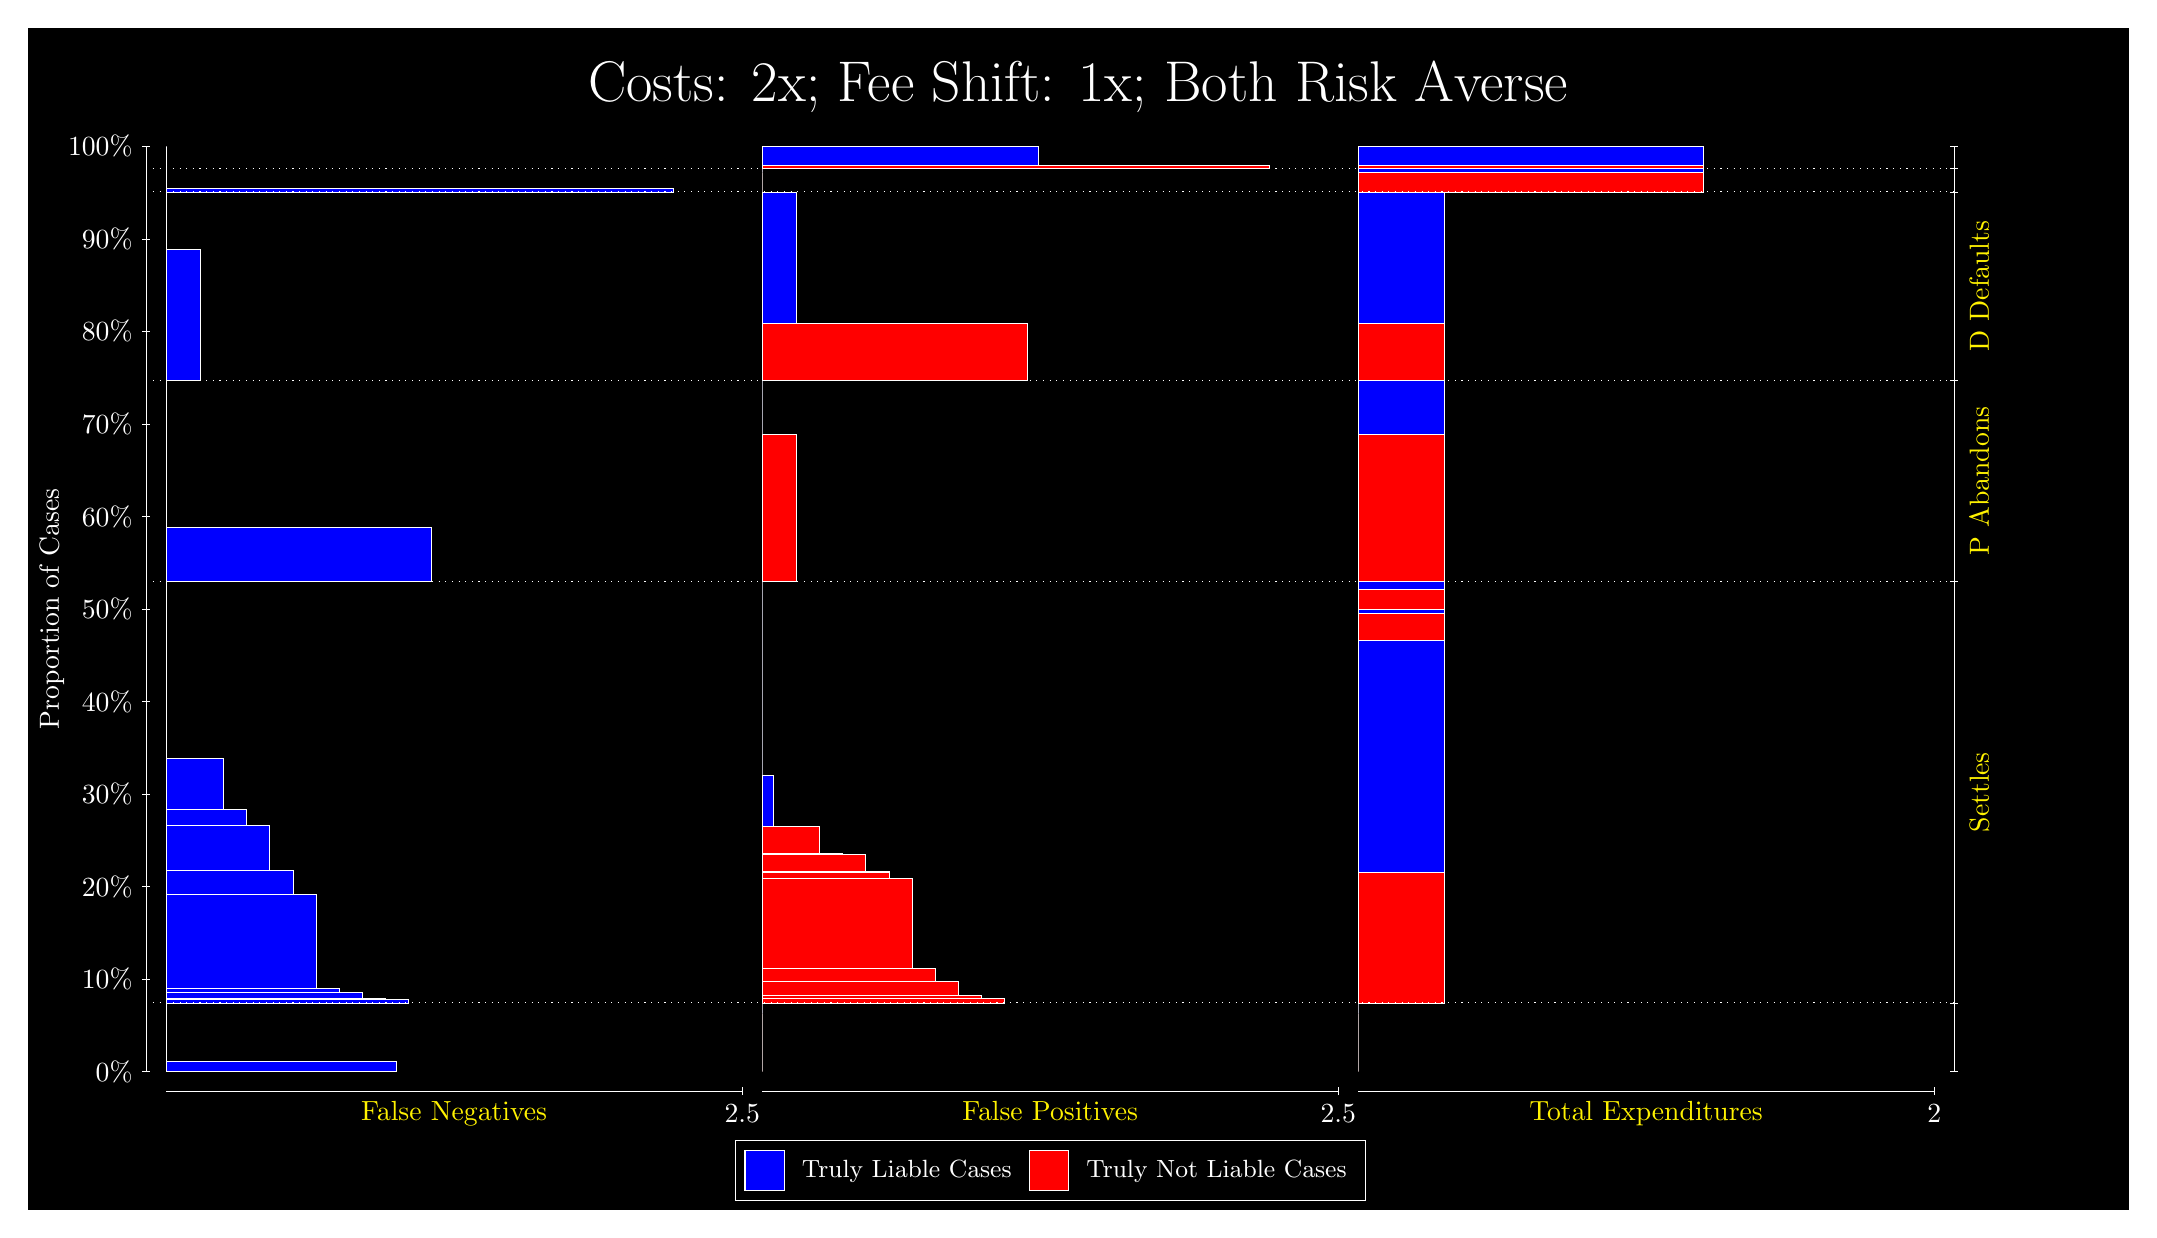
\begin{tikzpicture}
\draw[fill=black] (0,0) rectangle (26.667,15);
\draw[text=white] (0,13.5) rectangle (26.667,15) node[midway] {\huge Costs: 2x; Fee Shift: 1x; Both Risk Averse};
\draw[white, very thin] (1.5,1.75) -- (1.5,13.5);
\node[rotate=90, text=white, anchor=center] at (0.3, 7.625) {Proportion of Cases};
\draw[white, very thin] (1.45,1.75) -- (1.55,1.75);
\node[text=white, anchor=east] at (1.45, 1.75) {0\%};
\draw[white, very thin] (1.45,2.925) -- (1.55,2.925);
\node[text=white, anchor=east] at (1.45, 2.925) {10\%};
\draw[white, very thin] (1.45,4.1) -- (1.55,4.1);
\node[text=white, anchor=east] at (1.45, 4.1) {20\%};
\draw[white, very thin] (1.45,5.275) -- (1.55,5.275);
\node[text=white, anchor=east] at (1.45, 5.275) {30\%};
\draw[white, very thin] (1.45,6.45) -- (1.55,6.45);
\node[text=white, anchor=east] at (1.45, 6.45) {40\%};
\draw[white, very thin] (1.45,7.625) -- (1.55,7.625);
\node[text=white, anchor=east] at (1.45, 7.625) {50\%};
\draw[white, very thin] (1.45,8.8) -- (1.55,8.8);
\node[text=white, anchor=east] at (1.45, 8.8) {60\%};
\draw[white, very thin] (1.45,9.975) -- (1.55,9.975);
\node[text=white, anchor=east] at (1.45, 9.975) {70\%};
\draw[white, very thin] (1.45,11.15) -- (1.55,11.15);
\node[text=white, anchor=east] at (1.45, 11.15) {80\%};
\draw[white, very thin] (1.45,12.325) -- (1.55,12.325);
\node[text=white, anchor=east] at (1.45, 12.325) {90\%};
\draw[white, very thin] (1.45,13.5) -- (1.55,13.5);
\node[text=white, anchor=east] at (1.45, 13.5) {100\%};

\draw[white, very thin] (24.457,1.75) -- (24.457,13.5);
\draw[white, very thin] (24.407,1.75) -- (24.507,1.75);
\node[anchor=west] at (24.407, 1.75) {};
\draw[white, very thin] (24.407,2.6224) -- (24.507,2.6224);
\node[anchor=west] at (24.407, 2.6224) {};
\draw[white, very thin] (24.407,7.9742) -- (24.507,7.9742);
\node[anchor=west] at (24.407, 7.9742) {};
\draw[white, very thin] (24.407,10.526) -- (24.507,10.526);
\node[anchor=west] at (24.407, 10.526) {};
\draw[white, very thin] (24.407,12.921) -- (24.507,12.921);
\node[anchor=west] at (24.407, 12.921) {};
\draw[white, very thin] (24.407,13.215) -- (24.507,13.215);
\node[anchor=west] at (24.407, 13.215) {};
\draw[white, very thin] (24.407,13.5) -- (24.507,13.5);
\node[anchor=west] at (24.407, 13.5) {};

\draw[white, very thin, fill=blue] (1.75,1.75) rectangle (4.6775,1.8827);
\draw[white, very thin, fill=red] (1.75,1.8827) rectangle (1.75,2.6224);
\draw[white, very thin, fill=blue] (1.75,2.6224) rectangle (4.8239,2.6688);
\draw[white, very thin, fill=blue] (1.75,2.6688) rectangle (4.5312,2.674);
\draw[white, very thin, fill=blue] (1.75,2.674) rectangle (4.2384,2.7575);
\draw[white, very thin, fill=blue] (1.75,2.7575) rectangle (3.9457,2.8131);
\draw[white, very thin, fill=blue] (1.75,2.8131) rectangle (3.6529,3.9963);
\draw[white, very thin, fill=blue] (1.75,3.9963) rectangle (3.3602,4.2998);
\draw[white, very thin, fill=blue] (1.75,4.2998) rectangle (3.0674,4.8837);
\draw[white, very thin, fill=blue] (1.75,4.8837) rectangle (2.7746,5.0835);
\draw[white, very thin, fill=blue] (1.75,5.0835) rectangle (2.4819,5.7269);
\draw[white, very thin, fill=red] (1.75,5.7269) rectangle (1.75,7.9742);
\draw[white, very thin, fill=blue] (1.75,7.9742) rectangle (5.1167,8.659);
\draw[white, very thin, fill=red] (1.75,8.659) rectangle (1.75,10.526);
\draw[white, very thin, fill=blue] (1.75,10.526) rectangle (2.1891,12.194);
\draw[white, very thin, fill=red] (1.75,12.194) rectangle (1.75,12.921);
\draw[white, very thin, fill=blue] (1.75,12.921) rectangle (8.1906,12.966);
\draw[white, very thin, fill=red] (1.75,12.966) rectangle (1.75,13.215);
\draw[white, very thin, fill=red] (1.75,13.215) rectangle (1.75,13.261);
\draw[white, very thin, fill=blue] (1.75,13.261) rectangle (1.75,13.5);
\draw[white, very thin, fill=red] (9.3189,1.75) rectangle (9.3189,2.4897);
\draw[white, very thin, fill=blue] (9.3189,2.4897) rectangle (9.3189,2.6224);
\draw[white, very thin, fill=red] (9.3189,2.6224) rectangle (12.393,2.6769);
\draw[white, very thin, fill=red] (9.3189,2.6769) rectangle (12.1,2.7199);
\draw[white, very thin, fill=red] (9.3189,2.7199) rectangle (11.807,2.8932);
\draw[white, very thin, fill=red] (9.3189,2.8932) rectangle (11.515,3.0573);
\draw[white, very thin, fill=red] (9.3189,3.0573) rectangle (11.222,4.2004);
\draw[white, very thin, fill=red] (9.3189,4.2004) rectangle (10.929,4.2755);
\draw[white, very thin, fill=red] (9.3189,4.2755) rectangle (10.929,4.2986);
\draw[white, very thin, fill=red] (9.3189,4.2986) rectangle (10.636,4.5083);
\draw[white, very thin, fill=red] (9.3189,4.5083) rectangle (10.344,4.527);
\draw[white, very thin, fill=red] (9.3189,4.527) rectangle (10.051,4.8697);
\draw[white, very thin, fill=blue] (9.3189,4.8697) rectangle (9.4652,5.5131);
\draw[white, very thin, fill=blue] (9.3189,5.5131) rectangle (9.3189,7.9742);
\draw[white, very thin, fill=red] (9.3189,7.9742) rectangle (9.758,9.8415);
\draw[white, very thin, fill=blue] (9.3189,9.8415) rectangle (9.3189,10.526);
\draw[white, very thin, fill=red] (9.3189,10.526) rectangle (12.686,11.252);
\draw[white, very thin, fill=blue] (9.3189,11.252) rectangle (9.758,12.921);
\draw[white, very thin, fill=red] (9.3189,12.921) rectangle (9.3189,13.17);
\draw[white, very thin, fill=blue] (9.3189,13.17) rectangle (9.3189,13.215);
\draw[white, very thin, fill=red] (9.3189,13.215) rectangle (15.759,13.261);
\draw[white, very thin, fill=blue] (9.3189,13.261) rectangle (12.832,13.5);
\draw[white, very thin, fill=red] (16.888,1.75) rectangle (16.888,2.4897);
\draw[white, very thin, fill=blue] (16.888,2.4897) rectangle (16.888,2.6224);
\draw[white, very thin, fill=red] (16.888,2.6224) rectangle (17.986,4.2755);
\draw[white, very thin, fill=blue] (16.888,4.2755) rectangle (17.986,7.2281);
\draw[white, very thin, fill=red] (16.888,7.2281) rectangle (17.986,7.5708);
\draw[white, very thin, fill=blue] (16.888,7.5708) rectangle (17.986,7.6172);
\draw[white, very thin, fill=red] (16.888,7.6172) rectangle (17.986,7.8688);
\draw[white, very thin, fill=blue] (16.888,7.8688) rectangle (17.986,7.9742);
\draw[white, very thin, fill=red] (16.888,7.9742) rectangle (17.986,9.8415);
\draw[white, very thin, fill=blue] (16.888,9.8415) rectangle (17.986,10.526);
\draw[white, very thin, fill=red] (16.888,10.526) rectangle (17.986,11.252);
\draw[white, very thin, fill=blue] (16.888,11.252) rectangle (17.986,12.921);
\draw[white, very thin, fill=red] (16.888,12.921) rectangle (21.279,13.17);
\draw[white, very thin, fill=blue] (16.888,13.17) rectangle (21.279,13.215);
\draw[white, very thin, fill=red] (16.888,13.215) rectangle (21.279,13.261);
\draw[white, very thin, fill=blue] (16.888,13.261) rectangle (21.279,13.5);
\draw[white, dotted] (1.5,2.6224) -- (24.457,2.6224);
\draw[white, dotted] (1.5,7.9742) -- (24.457,7.9742);
\draw[white, dotted] (1.5,10.526) -- (24.457,10.526);
\draw[white, dotted] (1.5,12.921) -- (24.457,12.921);
\draw[white, dotted] (1.5,13.215) -- (24.457,13.215);
\draw[white, very thin] (1.75,1.5) -- (9.0689,1.5);
\node[text=yellow, anchor=north] at (5.4094, 1.5) {False Negatives};
\draw[white, very thin] (9.0689,1.45) -- (9.0689,1.55);
\node[text=white, anchor=north] at (9.0689, 1.45) {2.5};

\draw[white, very thin] (9.3189,1.5) -- (16.638,1.5);
\node[text=yellow, anchor=north] at (12.978, 1.5) {False Positives};
\draw[white, very thin] (16.638,1.45) -- (16.638,1.55);
\node[text=white, anchor=north] at (16.638, 1.45) {2.5};

\draw[white, very thin] (16.888,1.5) -- (24.207,1.5);
\node[text=yellow, anchor=north] at (20.547, 1.5) {Total Expenditures};
\draw[white, very thin] (24.207,1.45) -- (24.207,1.55);
\node[text=white, anchor=north] at (24.207, 1.45) {2};


\node[text=yellow, centered, rotate=90] at (24.777, 5.2983) {Settles};
\node[text=yellow, centered, rotate=90] at (24.777, 9.2502) {P Abandons};
\node[text=yellow, centered, rotate=90] at (24.777, 11.723) {D Defaults};



\draw (12.978300999999998,1.5) node[draw=none] (baseCoordinate) {};
\begin{scope}[align=center]
        \matrix[scale=0.5, draw=white, below=0.5cm of baseCoordinate, nodes={draw}, column sep=0.1cm]{
            \node[rectangle, draw, minimum width=0.5cm, minimum height=0.5cm, fill=blue] {}; &
            \node[draw=none, font=\small, text=white] (B) {Truly Liable Cases}; &
            \node[rectangle, draw, minimum width=0.5cm, minimum height=0.5cm, fill=red] {}; &
            \node[draw=none, font=\small, text=white] (B) {Truly Not Liable Cases}; \\
            };
\end{scope}

\end{tikzpicture}
\end{document}